% PGFPlots: multi-series line plot with error bars and shaded fill between curves
\documentclass{article}
\usepackage{pgfplots}
\pgfplotsset{compat=1.18}
\usepgfplotslibrary{fillbetween}

\begin{document}
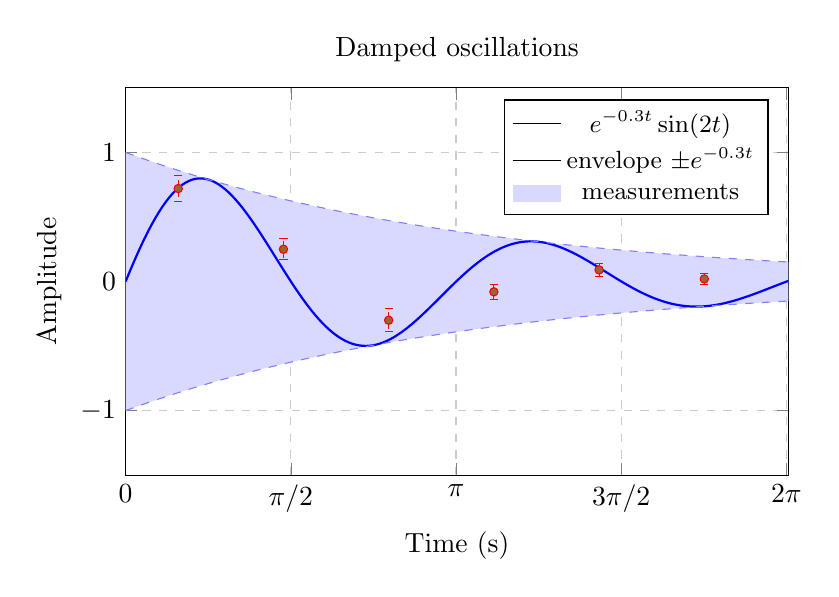
\begin{tikzpicture}
  \begin{axis}[
    width=10cm, height=6.5cm,
    xlabel={Time (s)},
    ylabel={Amplitude},
    xmin=0, xmax=6.3,
    ymin=-1.5, ymax=1.5,
    xtick={0,1.57,3.14,4.71,6.28},
    xticklabels={$0$,$\pi/2$,$\pi$,$3\pi/2$,$2\pi$},
    grid=major, grid style={dashed, gray!40},
    legend pos=north east,
    legend style={font=\small},
    title={Damped oscillations},
  ]
    % Envelope (fill between upper and lower)
    \addplot[name path=upper, draw=none, domain=0:6.3, samples=100]
      {exp(-0.3*x)};
    \addplot[name path=lower, draw=none, domain=0:6.3, samples=100]
      {-exp(-0.3*x)};
    \addplot[blue!15] fill between[of=upper and lower];

    % Main curve
    \addplot[blue, thick, domain=0:6.3, samples=200]
      {exp(-0.3*x)*sin(deg(2*x))};
    \addlegendentry{$e^{-0.3t}\sin(2t)$}

    % Envelope lines
    \addplot[blue!50, dashed, domain=0:6.3, samples=60]  { exp(-0.3*x)};
    \addplot[blue!50, dashed, domain=0:6.3, samples=60]  {-exp(-0.3*x)};
    \addlegendentry{envelope $\pm e^{-0.3t}$}

    % Sparse data points with error bars
    \addplot+[
      only marks, mark=*, mark size=1.5pt, red,
      error bars/.cd, y dir=both, y explicit,
    ] coordinates {
      (0.5, 0.72) +- (0, 0.10)
      (1.5, 0.25) +- (0, 0.08)
      (2.5,-0.30) +- (0, 0.09)
      (3.5,-0.08) +- (0, 0.06)
      (4.5, 0.09) +- (0, 0.05)
      (5.5, 0.02) +- (0, 0.04)
    };
    \addlegendentry{measurements}
  \end{axis}
\end{tikzpicture}
\end{document}
